\section{Magma migration}
For our very first simulation, we would like to simulate the 
production of magma in a simplified controlled scenerio.
I was inspired by the setup described previously in\cite{ModellingMeltingRates}.
The simulation will be setup in a chunk of rock ascending
with constant upwelling velocity.
A linear adiabatic temperature profile is applied here.
A linear intial rock composition is also applied here.

\subsection{Mathematical model}
We are going to show our coupled darcy-stokes semi-degenerate model
can solve this problem well.
In\cite{ModellingMeltingRates}, matrix creeping (Stokes equation) did not directly
involved in the simulation due to the fact that boundary condition restricts a 
constant background upwelling ascending velocity.
The solid matrix pressure is therefore strictly lithostatic pressure relating 
only to depth.
In\cite{ModellingMeltingRates}, only energy transports while concentration does not
participate in transport phenomenon. 

\begin{equation}
		  \begin{aligned}
					 \check{\bold{v}}_r + \phi_f^{1+\Theta}\nabla (\phi_f^{-1/2}\check{q}_f) &= 0\\
					 \phi_f^{-1/2}\nabla \cdot (\phi_f^{1+\Theta} \check{\bold{v}}_r) + \frac{1}{1-\phi_f}(\check{q}_f - \phi_f^{1/2}\check{q}) &=0 \\
					 \nabla \check{q} - \nabla \cdot \hat{\sigma}(\check{\bold{v}}_s) &= -(1-\phi_f)\hat{\bold{g}} \\
					 \nabla \cdot \check{\bold{v}}_s - \frac{\phi_f^{1/2}}{1-\phi_f}(\check{q}_f - \phi_f^{1/2}\check{q}) &= 0
		  \end{aligned}
\end{equation}

For simplification, we won't include diffusion into our transport model.
We drop the diffusion term here for the fact that diffusion coefficient is
relatively small compared to convective phenomenon. On the other hand, 
eutectic melting has a constant concentration such that gradient of 
concentration is of zero value. Hence the transport of component 2 (opx) 
can be expressed in terms of mixture theory as:
\begin{equation}
		  \begin{aligned}
					 \bar{C}_t + \nabla \cdot (\overline{C\bold{v}}) &= 0\\
					 \bar{C}_t + \nabla \cdot (\bold{v}_e^* \bar{C}) &= 0
		  \end{aligned}
\end{equation}
where $\bold{v}_e^*$ denotes effective veclocity 
$\bold{v}_e^* = \kappa \bold{v}_f + (1-\kappa)\bold{v}_s$
and $\kappa = \frac{\phi_f C_f}{\bar{C}}$ where $C_f$ and $\bar{C}$ using 
values from previous time step.
Enthalpy is transported in a similar manner.
\begin{equation}
		  \bar{\mathcal{H}}_t + \nabla \cdot (\overline{\mathcal{H}\bold{v}} - 
		  \bar{K}\nabla \mathcal{T})  = 0
\end{equation}

\subsubsection{Boundary conditions}
In order to solve the proposed darcy-stokes coupled equation, 
we need appropriate boundary condtions defined around the computational domain for stokes and darcy
subproblems.
The behavior of solid matrix is governed by Stokes equation.
Bernardi-raugel style element is used for this Stokes system, hence we need to provide
proper boundary conditions for two dofs per nodal and one additional supplemental 
flux bubble function for each edge dof.
The corresponding boundary condition are shown as follows.
\begin{itemize}
		  \item Prescribe essential boundary condition of constant upwelling ascending
					 velocity at supplying depth $z = z_0$ with $\bold{v}_s = \bold{W}$.
        \item Prescribe essential boundary condition to normal velocity and supplemental flux with the value of zero 
					 on two sides of the physical domain.
		  \item Prescribe zero traction (free dof) boundary condition (natural boundary condition) to tangantial 
					 velocity on two sides of the physical domain.
        \item Prescribe natural boundary conditoint to normal velocity and supplemental flux on the top side of
					 the physical domain representing a free outlet scenerio.
		  \item Prescribe essential boundary condition to tangential velocity with value zero on the top side of the physical domain.
\end{itemize}
The behavior do molten matrix is governed by Darcy equation.
We used BDM sytle element for this Darcy system, hence we just need to provide
proper boundary condition for each edges.
The corresponding boundary condition are shown as follows:
\begin{itemize}
        \item Prescribe zero values on two sides of the physical domain. 
        \item Prescribe zero values on the bottom of the physical domain representing no melting enters the
					 computational domain form bottom.
        \item Prescribe free (natural) boundary condition on the top of the physical domain representing
					 a free outlet of the melt.
\end{itemize}

\subsubsection{Initial conditions}
At the same time, we need an initial conditions for our transport equations.
In\cite{ModellingMeltingRates}, temperature and composition
are distributed linearly along against the depth. Unlike \cite{ModellingMeltingRates},
we implement eutectic melting model into our simulation. In our situation,
temperature and total composition won't be deterministic.
Here I make some modification on the setup.
Initially, the entire domain was burried under the partial melting region, where temperature was under the 
sub-solidus region.
Melting starts when the entire chunck ascending adiabatically. As pressure continuously lowering, 
the eutectic point is lowering at the same time. Hence, melting flux supplies from top. 

In eutectic melting situation, we cannot impose simple linear temperature directly due to 
the existence of the eutectic point. Therefore, an appropriate initial condition should be
assigned with careful selection.

Linear Enthalpy distribution (Near constant).
\begin{center}
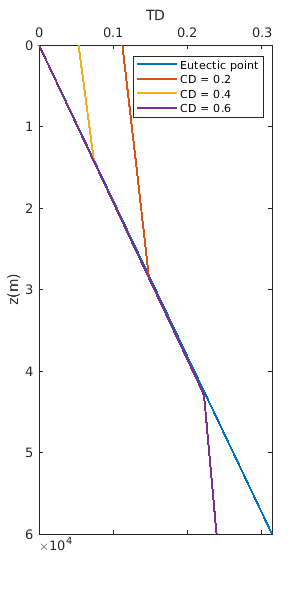
\includegraphics[width=5.5cm,height=10cm]{sections/pics/TDz_corrected}
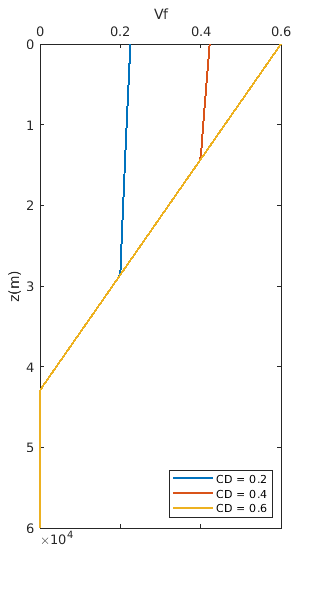
\includegraphics[width=5.5cm,height=10cm]{sections/pics/Vfz_corrected}
\end{center}

%Using enthalpy and composition distribution calculated above,
%we can generate corresponding initial velocity distribution:
%\begin{center}
%
\includegraphics[width=5.5cm,height=10cm]{sections/pics/stokes}
%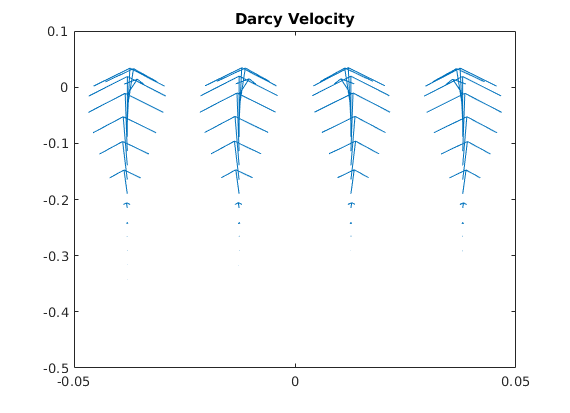
\includegraphics[width=5.5cm,height=10cm]{sections/pics/darcy}
%\end{center}
%!!!Corrected version
%\begin{center}
%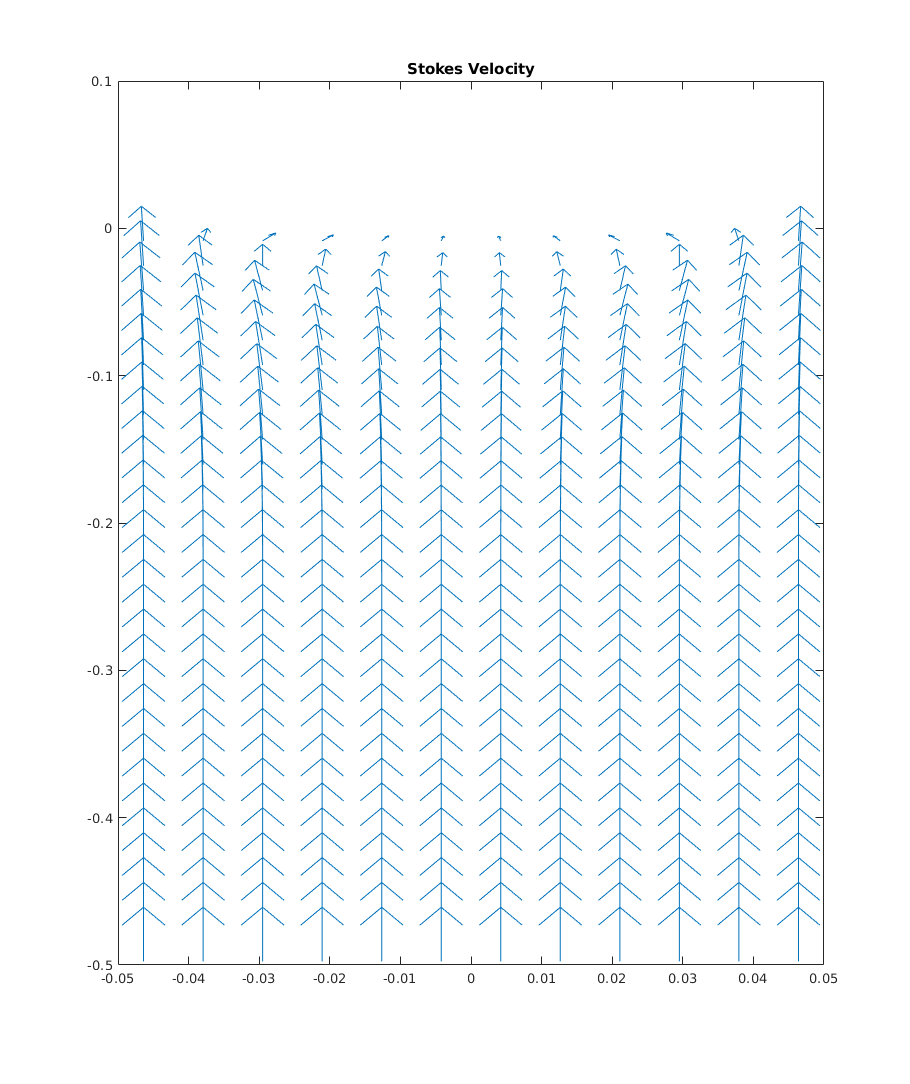
\includegraphics[width=5.5cm,height=10cm]{sections/pics/stokesv}
%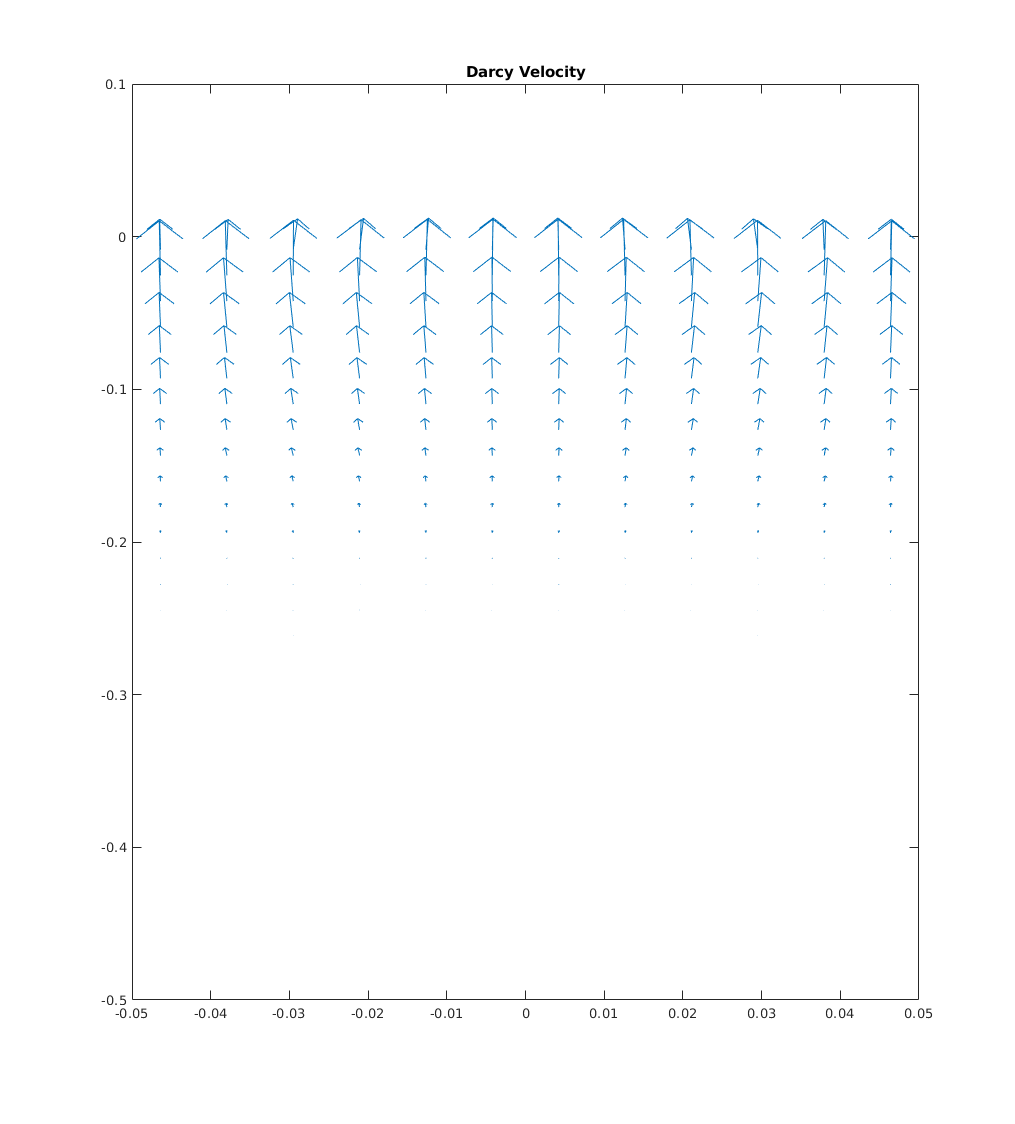
\includegraphics[width=5.5cm,height=10cm]{sections/pics/darcyv}
%\end{center}
%
%\begin{center}
%
\includegraphics[width=5.5cm,height=10cm]{sections/pics/test1/darcyv}
%
\includegraphics[width=5.5cm,height=10cm]{sections/pics/test1/stokesv}
%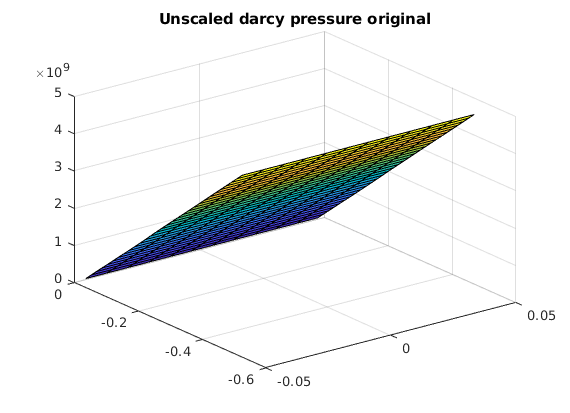
\includegraphics[width=5.5cm,height=10cm]{sections/pics/test1/darcyp}
%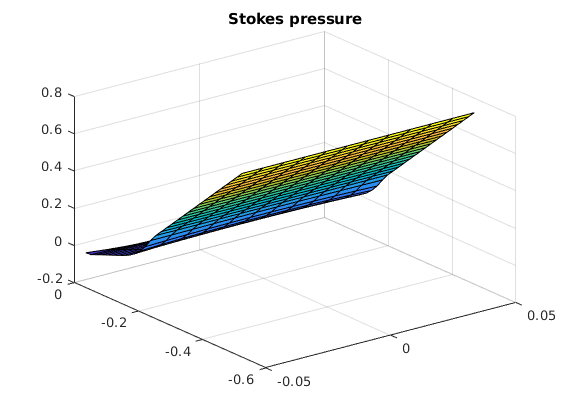
\includegraphics[width=5.5cm,height=10cm]{sections/pics/test1/stokesp}
%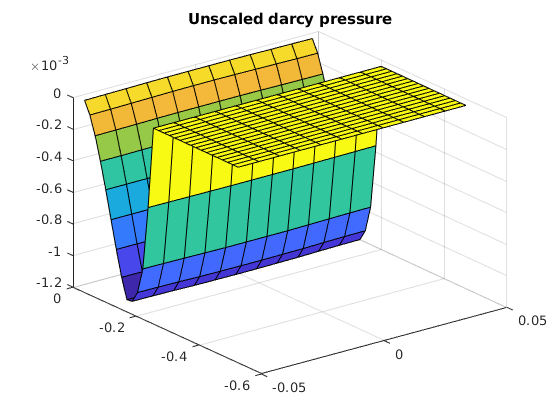
\includegraphics[width=5.5cm,height=10cm]{sections/pics/test1/uscaleddarcyp}
%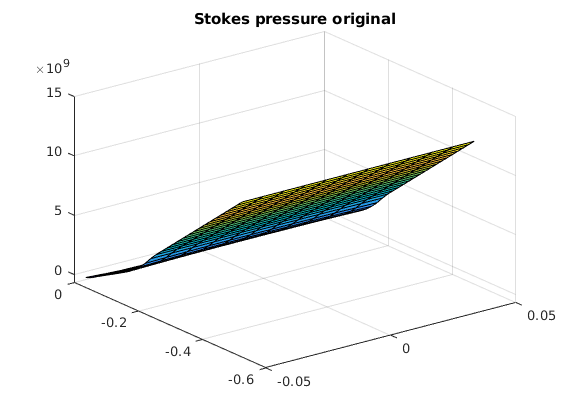
\includegraphics[width=5.5cm,height=10cm]{sections/pics/test1/stokespori}
%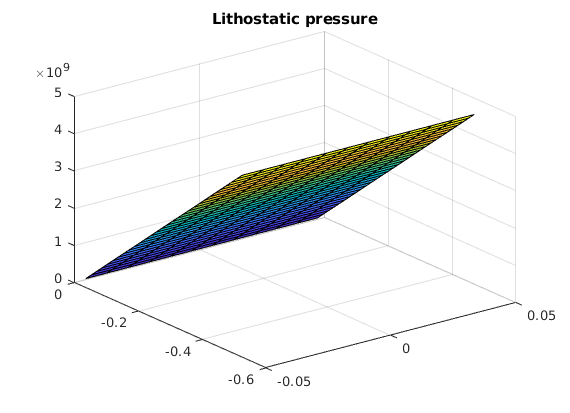
\includegraphics[width=5.5cm,height=10cm]{sections/pics/test1/litho}
%\end{center}
%
\subsubsection{Melting depth}
As the magma chunk ascending adiabatically, we can define a depth $z_m$ where melting
starts. From the plots above, we can conclude that in our model
\begin{itemize}
\item Change of dimensionless composition can only affect the separaration of eutection and super-eutection region.
\item Change of dimensionless composition will not affect where magam leave eutection melting region.
\end{itemize}
A fixed melting depth can therefore be calculated despite dimensionless composition distribution.
The melting happens when current temperature reaches the eutectic melting temperature.
In the situtation of linear dimensionless enthalpy distribution $f(HD) = HD_0 + \eta z$.
Assuming lithostatic pressure distribution, the eutectic point at given depth $z$ is: $\mathcal{T}_e = 0 + \gamma *\rho_s g z$.
The melting depth is therefore calculated as: $z = \frac{HD_0}{\rho_s g - \eta}$.
In this case, the smaller initial dimensionless enthalpy $HD_0$ the shorter melting depth.

\subsection{Interpolation of stokes pressure}
We are using piece-wise constant L2 approximation space for stokes and darcy pressure.
In order to evaluate point-wise pressure. We are going to present an interpolation using
generated piece-wise constant pressure.

\subsection{Approximation of physical values on the cell edges}
In the process of simulation, plenty of physical values are defined on the gauss points of cell edges.
Take $\kappa$ for example, where $\kappa = \frac{\phi_f c_f}{\bar{c}}$, two phase parameters $\phi_f$ 
and $c_f$ are computed with phase package using reconstructed values on both side of the cell edges.
The value of $\bar{c}$ are directly obtained by WENO reconstruction. Therefore, two different values
$\kappa_{In}$ and $\kappa_{Out}$ will be obtained during this computation process, which will be 
used in the calculation of the numerical flux.

\subsection{Nondimensionalization and reterive of original physical variables}
We converting scaled and nondimensionalized computational variables back to original physical variables.
Note, the characteristic length defined similarly to the definition of compact length.
\begin{equation*}
\tilde{\bold{v}}_r = \phi^{-1-\Phi}\bold{u} \quad \text{,} \quad \tilde{q}_f = \phi^{1/2} q_f \quad \text{and} \quad  q = q_s + \phi(q_f - q_s)
\end{equation*}
while the pressure potentials are defined as
\begin{equation*}
q_f = p_f - \rho_fgz \quad \text{and} \quad q_s = p_s - \rho_f g z
\end{equation*}
and we define reference physical variables as:
\begin{equation*}
l_0 = (\frac{k_0 \mu_s}{\mu_f})^{1/2} \quad \text{and} \quad q_0 = \rho_r g l_0 \quad \text{and} \quad w = \frac{k_0 \rho_r g}{\mu_f}
\end{equation*}
Hence we can reterive the two original physical pressure as:
\begin{equation*}
\begin{aligned}
p_f &= q_0 \hat{q}_f + \rho_f g z\\
p_s &= \frac{\hat{q} - \phi\hat{q}_f}{1-\phi} q_0 + \rho_f g z
\end{aligned}
\end{equation*}
where $\hat{q}$ and $\hat{q}_f$ are dimensionless variables computed in the linear system.
\begin{center}
\begin{tabular} {c| c| c| c}
\text{Scale} & \text{Definition} & \text{Typical value} & \text{Units} \\
\hline
$V_0$ & \quad & 3.2 & $\text{cm y}^{-1}$ \\
$l_0$ & $(\frac{k_0 \mu_s}{\mu_f})^{1/2}$ & \\ 
\hline
\end{tabular}
\end{center}
